\documentclass[12pt]{article}
\usepackage{amsmath,amsfonts}
\usepackage{enumerate}
\usepackage{graphicx}
\usepackage{float}
\usepackage{multirow}
\usepackage{booktabs}
\usepackage{placeins}

\renewcommand{\baselinestretch}{1}
\topmargin 0in \headheight 0.0in \textheight 9in \textwidth 6.5in
\oddsidemargin 0.1in \evensidemargin 0.1in

\graphicspath{{/Users/siyangren/Documents/ra-cida/ESFGSP_Paper/Simulations/results/figures}}


\title{}
\author{Siyang Ren, Nichole E. Carlson, William Lippitt, Yue Wang}
\date{}

\begin{document}

\maketitle

\section*{Notes}

\begin{itemize}
  \item In the Data Simulation section, I am using Moran's eigenvectors instead of the default eigenvectors to project pixels into the frequency domain. Is this correct? Additionally, I need to confirm that \( \mathbf{E} \) is orthogonal. Orthogonality is necessary to ensure that \( \mathbf{E}^T \mathbf{C} \mathbf{E} \) results in a diagonal matrix.
\end{itemize}

\section*{Introduction}

This study involves two simulations aimed at evaluating the performance of LASSO models in identifying significant features in high-dimensional datasets. The first simulation assumes sparsity in the pixel space, where each feature corresponds to a pixel, while the second simulation assumes sparsity in the frequency domain, which is a transformation of the pixel space.

The pixel space represents the original high-dimensional domain where correlations among features may exist. The frequency space, derived through eigen decomposition, represents the data in terms of its frequency components.


\section*{Methods}

\subsection*{Data Simulation}

Let \( \mathbf{x} \) be a column vector representing the pixel values of a single observation, with \( n = 256 \) pixels in total. The covariance matrix \( \mathbf{C} \) is defined by an exponential correlation structure: 
\[
\mathbf{C}_{ij} = -\exp(\operatorname{dist}(i,j))
\]
where \( \operatorname{dist}(i,j) \) is the distance between pixels \( i \) and \( j \) on a \( 16 \times 16 \) grid. Define \( \mathbf{M} = \mathbf{I} - \mathbf{1} \mathbf{1}^{\prime} / n \) as a centering matrix. We decompose \( \mathbf{MCM} \) as
\[
\mathbf{MCM} = \mathbf{E}_{\text{full}} \mathbf{\Lambda}_{\text{full}} \mathbf{E}_{\text{full}}^{\prime}
\]
where \( \mathbf{E}_{\text{full}} \) is the matrix of eigenvectors [the notations above come from reference 1]. We transform the vector \( \mathbf{x} \) into the frequency space using:
\[
\mathbf{x}_{\text{freq}} = \mathbf{E}^T \mathbf{x}
\]
The covariance matrix of \( \mathbf{x}_{\text{freq}} \) becomes \( \mathbf{E}^T \mathbf{C} \mathbf{E} \), which is diagonal by construction [diagonal needs to be verified].

In each simulation, \( \mathbf{X} \) denotes the matrix of all observations, where each row represents an observation, and there are 1000 observations in total. The relationship between \( \mathbf{X} \) and \( \mathbf{X}_{\mathrm{freq}} \) is:
\[
\mathbf{X}_{\mathrm{freq}} = \mathbf{X} \mathbf{E}
\]

Next, we define the coefficient vectors in both spaces. Let \( \boldsymbol{\beta} \) be the coefficient vector in the pixel space and \( \mathbf{b} \) in the frequency space. To ensure \( \mathbf{X} \boldsymbol{\beta} = \mathbf{X}_{\mathrm{freq}} \mathbf{b} \), we require:
\[
\boldsymbol{\beta} = \mathbf{E} \mathbf{b}
\]

Two scenarios are simulated:

\begin{enumerate}
  \item \textbf{Pixel space sparsity:} In this scenario, \( \boldsymbol{\beta} \) is sparse, with non-zero values confined to a central \( 8 \times 8 \) region. The covariate matrix \( \mathbf{X} \) is generated from a multivariate normal distribution with zero mean and covariance matrix \( \mathbf{C} \). The response variable \( \mathbf{y} \) is drawn from a binomial distribution, with the success probability determined by \( \boldsymbol{\eta} = \mathbf{X} \boldsymbol{\beta} \). The non-zero entries of \( \boldsymbol{\beta} \) are constant and chosen such that the probability \( \mathbf{p} = \frac{1}{1 + \exp(-\boldsymbol{\eta})} \) is uniformly distributed in \( [0, 1] \).
  \item \textbf{Frequency space sparsity:} In this case, \( \mathbf{b} \) is sparse, with 10\% of its 256 entries randomly set to non-zero values, while the rest remain zero. The covariate matrix \( \mathbf{X}_{\mathrm{freq}} \) is generated from a multivariate normal distribution with zero mean and a diagonal covariance matrix, assuming the eigenvalues decrease along the diagonal [I am thinking of what step size is proper, currently using constant step size]. The non-zero entries in \( \mathbf{b} \) are constant and chosen such that \( \mathbf{p} \) is uniformly distributed in \( [0, 1] \), and the response variable \( \mathbf{y} \) is drawn from a binomial distribution with probability \( \mathbf{p} \).
\end{enumerate}

After simulating data from either space, the values in the other space are calculated using the transformations described above. Note that when simulating data from the frequency space, even though the diagonal covariance matrix is randomly chosen, not calculated by \( \mathbf{E}^T \mathbf{C} \mathbf{E} \), we still use \( \mathbf{E} \) to transform it back to the pixel space.

\subsection*{Model Evaluation}

To evaluate the performance of LASSO in both spaces, we fit two models: one using covariates in the pixel space and another using covariates in the frequency space. To select the optimal regularization parameter \( \lambda \), the dataset is split into training (80\%) and test (20\%) sets. The regularization parameter \( \lambda \) is tuned using cross-validation based on the binomial deviance metric, with the dataset divided into 10 folds. Two values of \( \lambda \) are considered: \texttt{lambda.min}, which minimizes the cross-validated error, and \texttt{lambda.1se}, which represents the largest \( \lambda \) within one standard error of the minimum.

For each iteration, model performance is evaluated using the selected \( \lambda \) on the test set. The evaluation metrics include accuracy, Area Under the Curve (AUC), and p-values for each covariate. P-values are calculated using the \texttt{hdi} package [provide more details on how this package calculates p-values]. The simulation is repeated 500 times, and we report the mean and standard deviation of accuracy and AUC. For p-values, we report the percentage of instances where \( p < 0.05 \) at each location [I am wondering whether we need to do adjustment here].


\section*{Results}

\subsection*{Effect Size Determination}

In Simulation 1, the distribution of the success probability \( \mathbf{p} \) was evaluated at various non-zero values for \( \boldsymbol{\beta} \): 0.01,
0.05, 0.1, 0.2, and 1. As shown in Figure \ref{fig:sim1_p_dist}, 0.1 yielded the most uniform distribution
of \( \mathbf{p} \), making it the optimal choice for model fitting. Similarly, in Simulation 2, the distribution of \( \mathbf{p} \) was assessed at various non-zero values for \( \mathbf{b} \): 0.1, 0.2, 0.4, 0.6, 0.8, and 1. As illustrated in Figure \ref{fig:sim2_p_dist}, 0.2 resulted in the most uniform distribution of \( \mathbf{p} \).

\begin{figure}[h!]
	\centering
	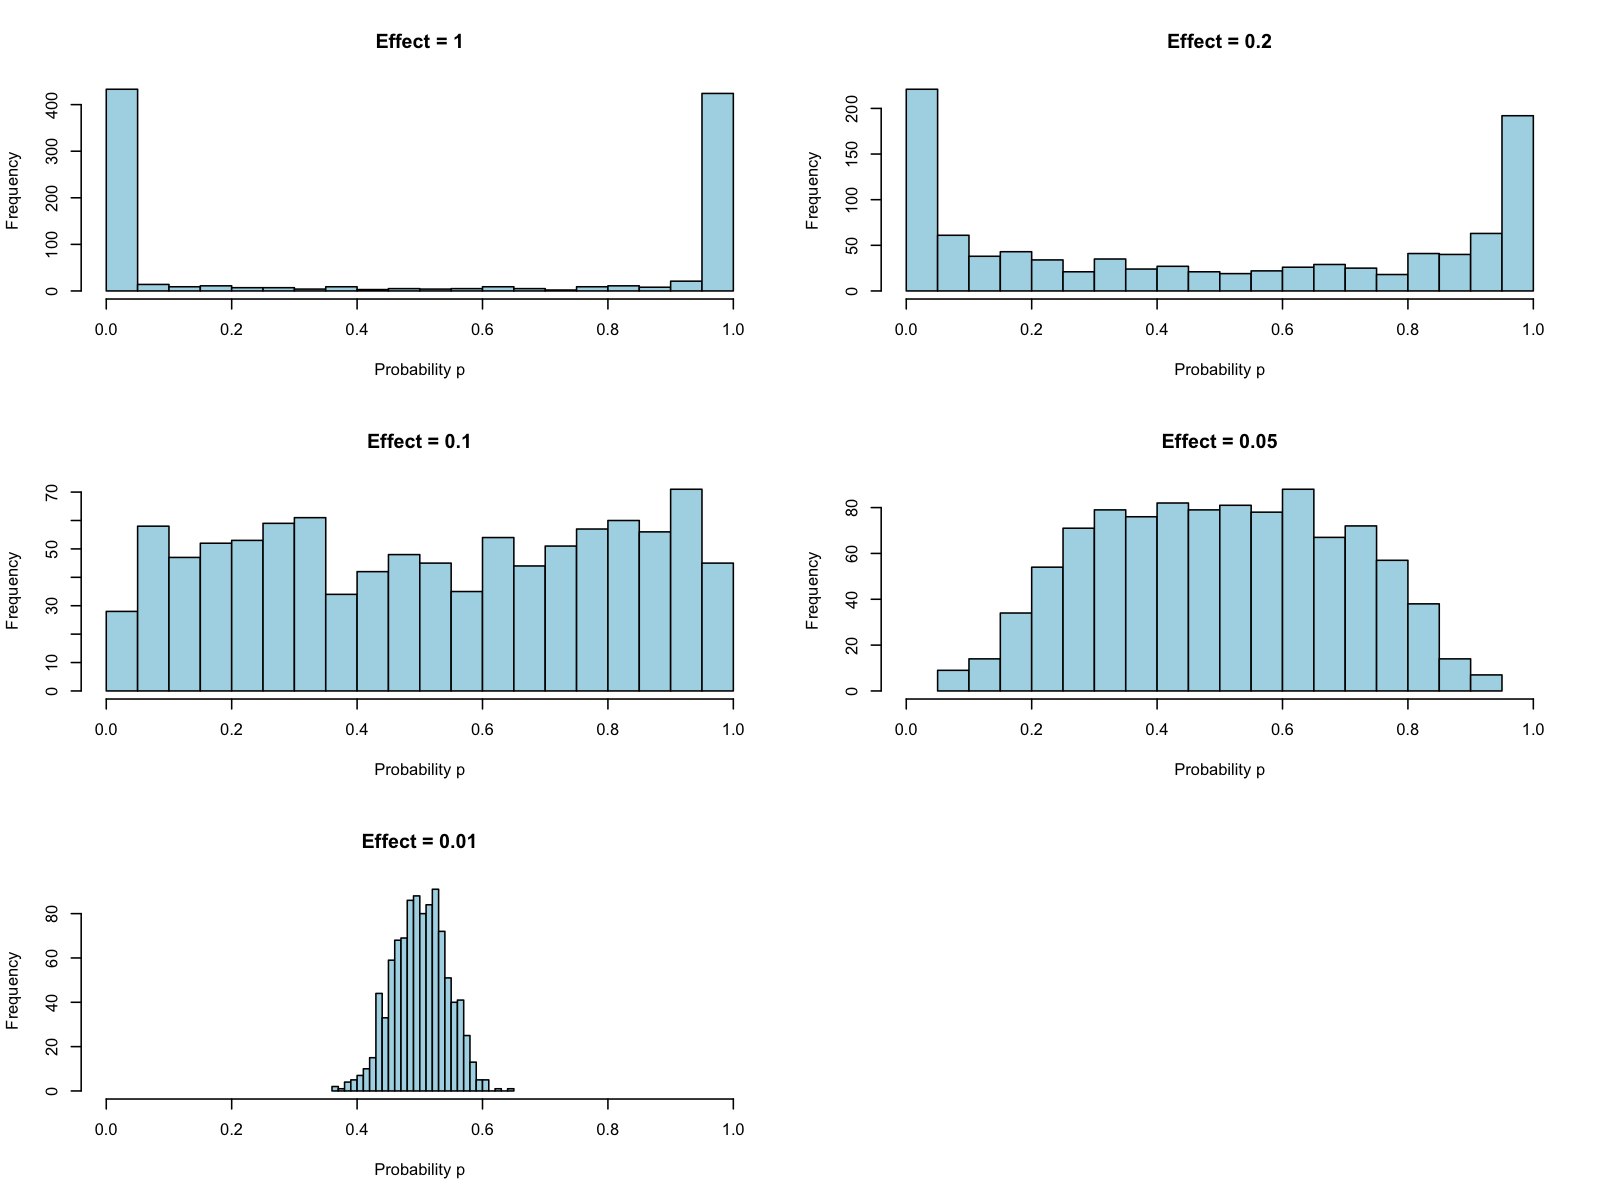
\includegraphics[width=0.8\textwidth]{sim1_p_dist.png}
	\caption{Distribution of success probability \( p \) at different \( \beta \) values in Simulation 1.}
	\label{fig:sim1_p_dist}
\end{figure}

\begin{figure}[h!]
	\centering
	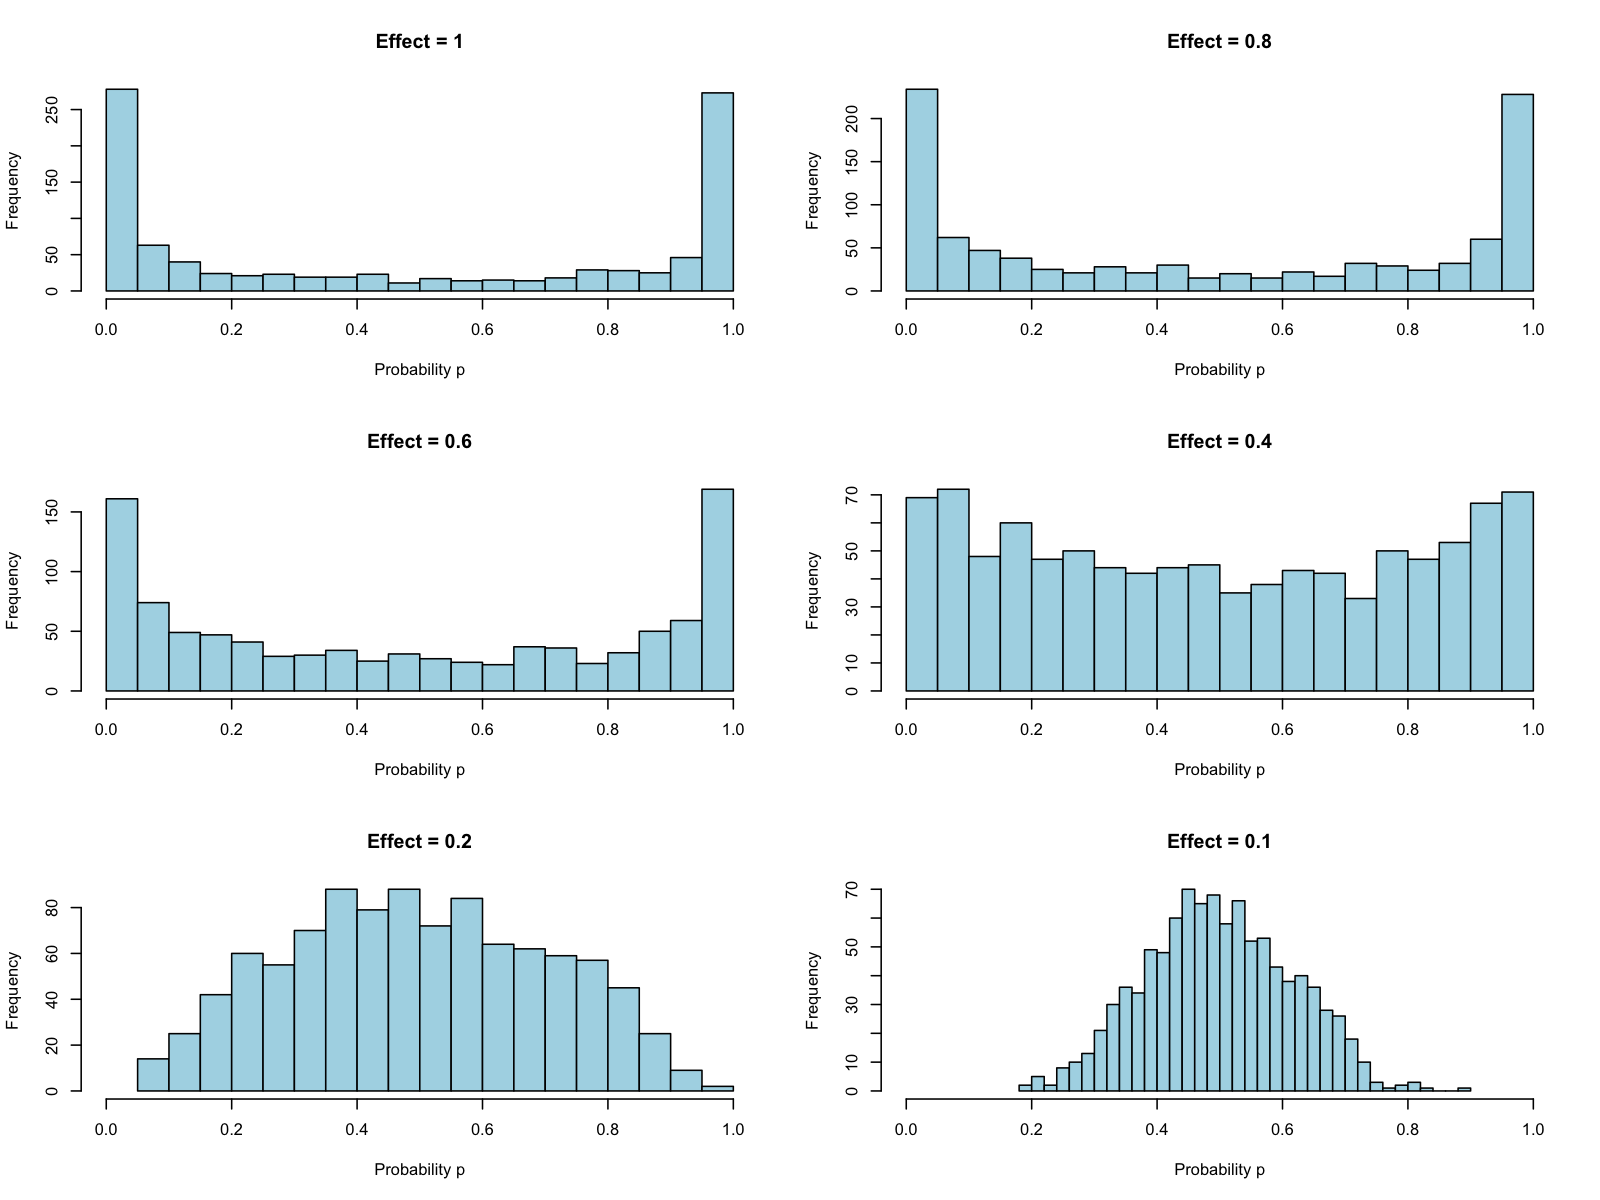
\includegraphics[width=0.8\textwidth]{sim2_p_dist.png}
	\caption{Distribution of success probability \( p \) at different \( b \) values in Simulation 2.}
	\label{fig:sim2_p_dist}
\end{figure}

\FloatBarrier

\subsection*{Group Mean Difference}

Figure \ref{fig:group_diff1} shows the group mean difference in covariate values between instances where \( y = 1 \) and \( y = 0 \) for Simulation 1. The difference in \( \boldsymbol{\beta} \) (left) is shown in heatmap as the location matters, and the difference in \( \mathbf{b} \) are shown by a scatterplot, where the x-axis is standardized order of eigenvalues, with the larger eigenvalues have larger values, and y-axis as the group means for the coefficients. Figure \ref{fig:coefs_sim1} shows the actual coefficient values we used in the same simulation. We can see that the group mean difference in positions where the actual coefficient value is non-zero is larger, which makes sense as covariates with larger values have higher probabilities to be assigned to \( y = 1 \).

Figure \ref{fig:group_diff2} and \ref{fig:coefs_sim2} show the similar figures for Simulation 2, where coefficient vectors in the frequency space is specified and transformed to the pixel space. I feel that the group mean difference showing in the heatmap still show similar patterns compared to the actual values, I do notice some locations have different directions, like a shadow blue compared to a shallow red. But actual values have a large absolute value do keep the same direction in the group mean diff figure. The interesting finding comes to the scatterplots. We can see that the actual non-zero values are a constant 0.2, but the estimated values are up and down around 0, and goes larger (with larger variance) for those corresponding to larger eigenvalues. The larger variance makes sense to me, as the covariance matrix I used is a diagonal matrix with decreasing diagonal values. Even though all coefficients are zero, the group mean difference should be scattered around 0 and has larger variance along the x-axis. What surprise me is that I didn't see clear pattern showing which location has non-zero values. I am guessing the non-zero effect is relative small compared to the covariance I specified [maybe next step].

\begin{figure}[h!]
	\centering
  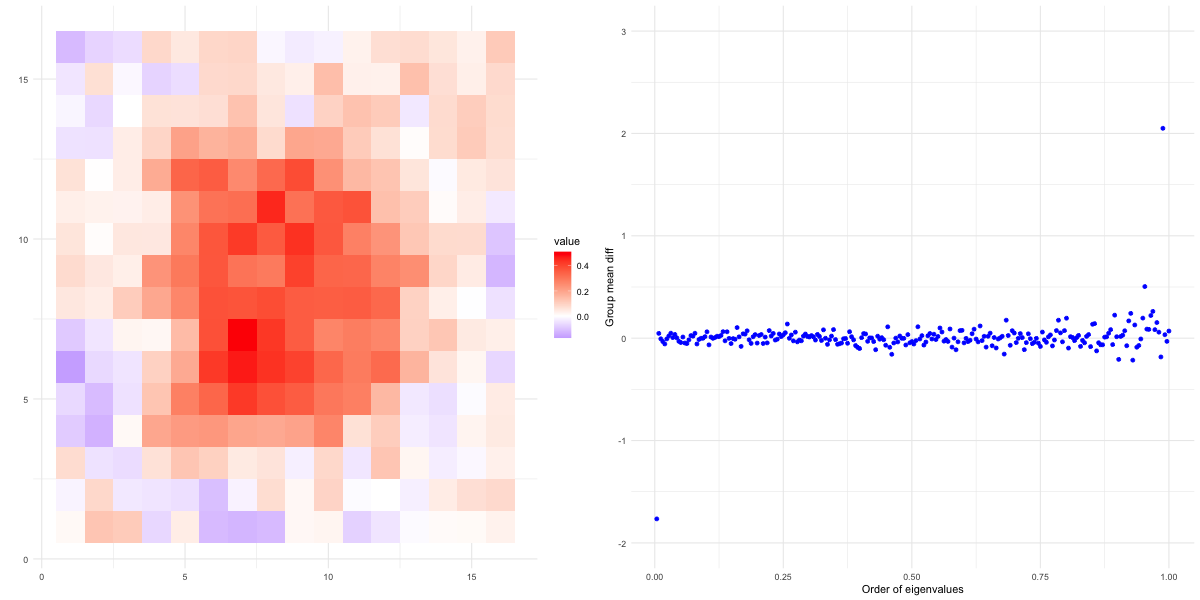
\includegraphics[width=0.8\textwidth, height=0.35\textwidth]{group_mean_diff_sim1.png}
	\caption{Group mean difference in covariate values between instances where \( y = 1 \) and \( y = 0 \) in Simulation
		1, shown for both the pixel space (left) and frequency space (right).}
	\label{fig:group_diff1}
\end{figure}

\begin{figure}[h!]
	\centering
	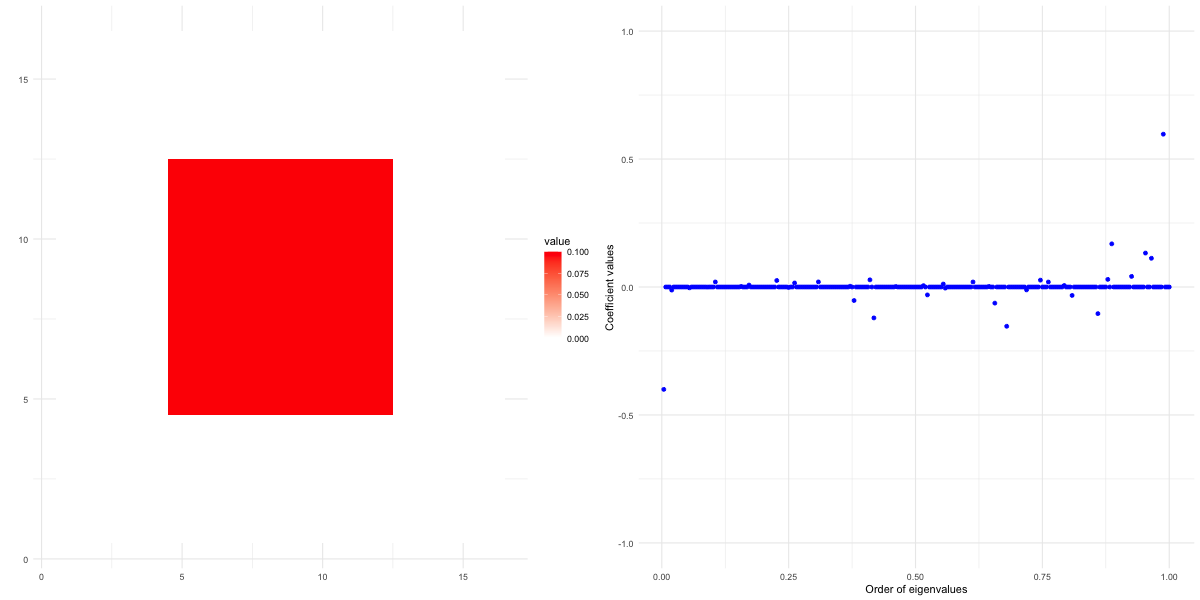
\includegraphics[width=0.8\textwidth, height=0.35\textwidth]{actual_coefs_sim1.png}
	\caption{Actual coefficients in Simulation 1 for the pixel space (left) and frequency space (right).}
	\label{fig:coefs_sim1}
\end{figure}

\begin{figure}[h!]
	\centering
	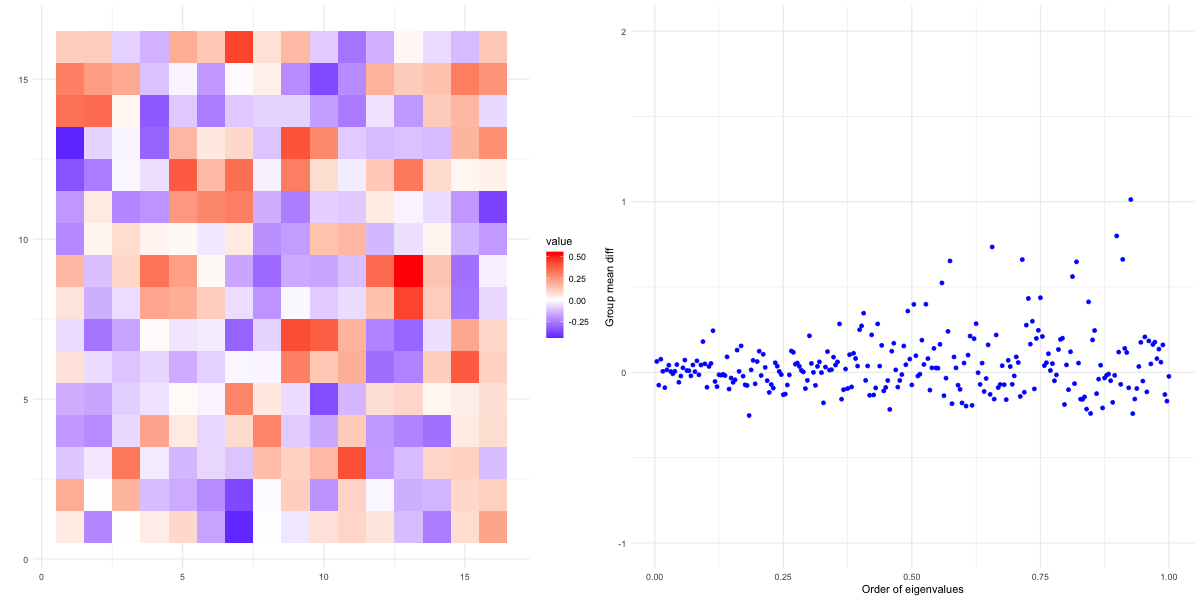
\includegraphics[width=0.8\textwidth, height=0.35\textwidth]{group_mean_diff_sim2.png}
	\caption{Group mean difference in covariate values between instances where \( y = 1 \) and \( y = 0 \) in Simulation 2.}
	\label{fig:group_diff2}
\end{figure}

\begin{figure}[h!]
	\centering
	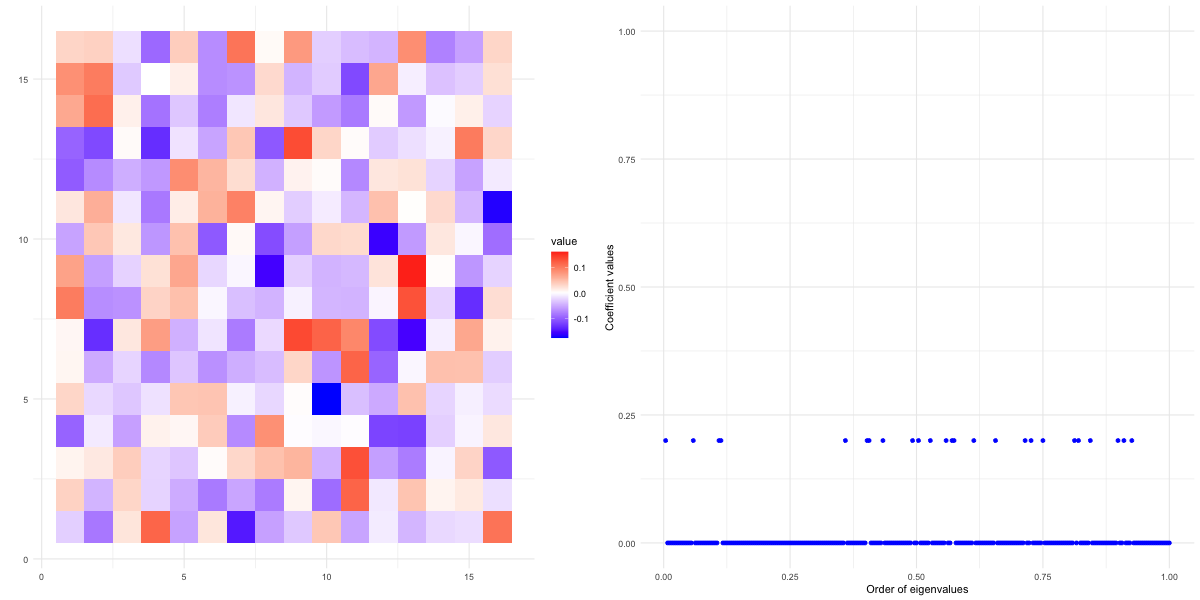
\includegraphics[width=0.8\textwidth, height=0.35\textwidth]{actual_coefs_sim2.png}
	\caption{Actual coefficients in Simulation 2 for the pixel space (left) and frequency space (right).}
	\label{fig:coefs_sim2}
\end{figure}

\FloatBarrier

\subsection*{AUC and Accuracy}

Table~\ref*{tab:auc_acc_table} presents the average AUCs and accuracies over the 500 iterations. Regardless of whether
sparsity is assumed in the pixel space (Simulation 1) or the frequency space (Simulation 2), models fitted in the
frequency space consistently outperformed those fitted in the pixel space. Specifically, in Simulation 1, using
\texttt{lambda.min} as the regularization value, models fitted with covariates from the pixel space achieved an AUC of
0.803 (SE = 0.031) and an accuracy of 72.6\% (SE = 0.032). In contrast, models fitted with covariates from the
frequency space achieved a slightly higher AUC of 0.826 (SE = 0.028) and a higher accuracy of
74.5\% (SE = 0.030). A similar trend was observed in Simulation 2, with models fitted in the frequency space
demonstrating superior performance regardless of the regularization parameter used.

\begin{table}[h!]
	\centering
	\caption{Comparison of AUC and accuracy between models fitted in the pixel space and frequency space across 500 iterations for Simulation 1 and Simulation 2.}
	\label{tab:auc_acc_table}
	\begin{tabular}{l|cc|cc}
		\toprule
		\textbf{Simulation}   & \multicolumn{2}{c}{\textbf{Model in Pixel Space}} & \multicolumn{2}{c}{\textbf{Model in Frequency Space}}                                              \\
		\midrule
		                      & \textbf{AUC (SE)}                                 & \textbf{Accuracy (SE)}                                & \textbf{AUC (SE)} & \textbf{Accuracy (SE)} \\
		\midrule
		\textbf{Simulation 1} &                                                   &                                                       &                   &                        \\
    \texttt{lambda.min}            & 0.803 (0.031)                                     & 0.726 (0.032)                                         & 0.826 (0.028)     & 0.745 (0.030)          \\
      \texttt{lambda.1se}            & 0.800 (0.032)                                     & 0.722 (0.032)                                         & 0.826 (0.029)     & 0.745 (0.031)          \\
		\midrule
		\textbf{Simulation 2} &                                                   &                                                       &                   &                        \\
    \texttt{lambda.min}            & 0.755 (0.036)                                     & 0.684 (0.034)                                         & 0.812 (0.030)     & 0.732 (0.032)          \\
      \texttt{lambda.1se}            & 0.735 (0.039)                                     & 0.669 (0.038)                                         & 0.812 (0.031)     & 0.732 (0.032)          \\
		\bottomrule
	\end{tabular}
\end{table}

\subsection*{Coefficients Estimation}

The mean estimated coefficients across iterations were calculated. Figure \ref{fig:beta_estimates} displays the mean estimated \( \beta \) values. There are two conclusions here: 1. Using \texttt{lambda.min} and \texttt{lambda.1se} makes no significant difference in the coefficients estimated. 2. The estimated values aligns well with the actual values.

Figure \ref{fig:b_estimates} presents the mean estimated \( b \) values plotted against the order of eigenvalues. The order of eigenvalues are calculated the same way as above. For Simulation 1, \texttt{lambda.1se} shrinks the estimated coefficients more than \texttt{lambda.min}, as it provides a larger panelty on it. For Simulation 2, even though it is not obvious, I feel the estimated values has an increase trend as the eigenvalues increase. [Still, I am wondering whether this is related to the covariance matrix, the decreased diagonal values, consider math proof?].

\begin{figure}[h!]
	\centering
	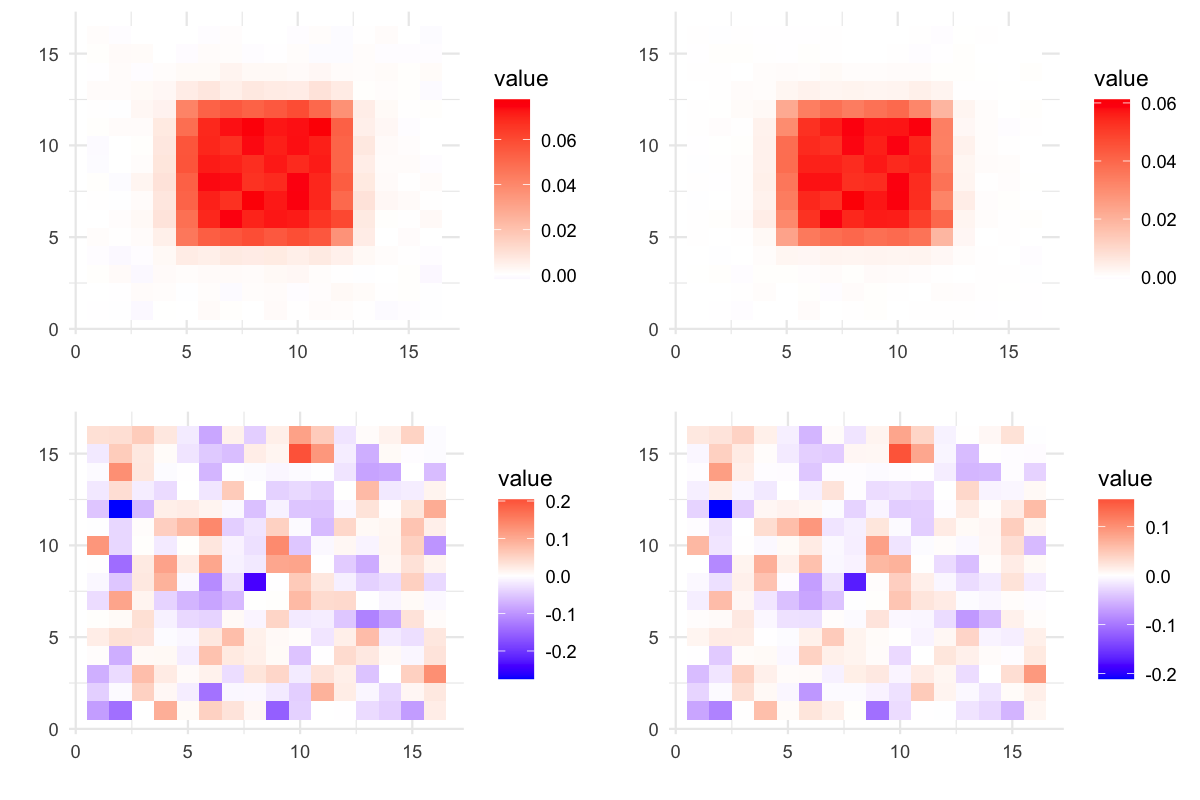
\includegraphics[width=0.8\textwidth]{beta_estimates.png}
	\caption{Mean estimated \( \beta \) values across simulations, with models fitted using \texttt{lambda.min} (left) and
		\texttt{lambda.1se} (right). The top row shows results for Simulation 1, while the bottom row shows results for Simulation 2.}
	\label{fig:beta_estimates}
\end{figure}

\begin{figure}[h!]
	\centering
	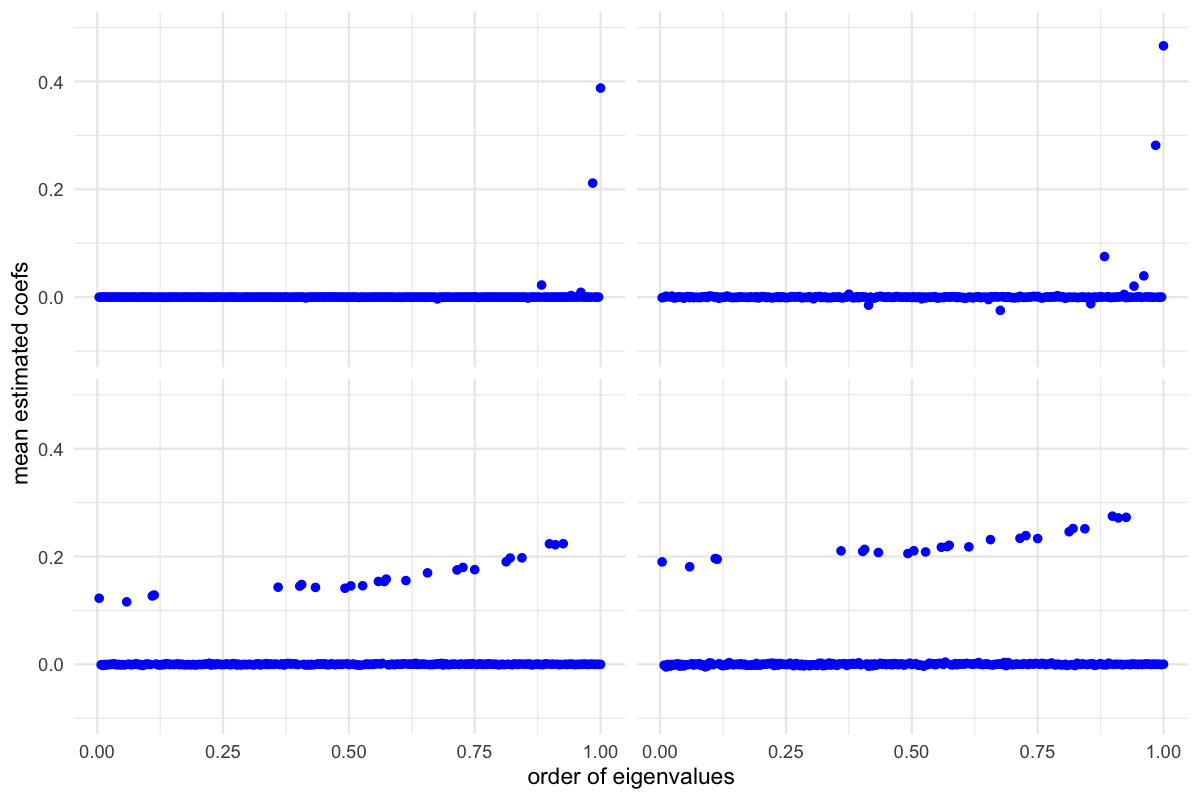
\includegraphics[width=0.8\textwidth]{b_estimates.png}
	\caption{Mean estimated \( b \) values across simulations, plotted against ordered eigenvalues. Models fitted using
		\texttt{lambda.min} are on the left and models fitted with \texttt{lambda.1se} on the right. The top row shows results for Simulation 1, while the bottom row shows results for Simulation 2.}
	\label{fig:b_estimates}
\end{figure}

\FloatBarrier

\subsection*{Significant P-values}

It is interesting to notice that the even though the heatmap for significance of \( \boldsymbol{\beta} \) in Simulation 1 follows the pattern of the actual non-zero values, the percentage of significance is relative low (Figure \ref{fig:perc_sign_beta} left) compared to the percentage for \( \mathbf{b} \) (Figure \ref{fig:perc_sign_b} left), where the non-zero values have as high as 100\% significance across iterations.  

Another finding is that, again, even though the non-zero effect size for \( \mathbf{b} \) is a constant number in simulation 2, the percentage of significance has an increase trend as eigenvalues increase (Figure \ref{fig:perc_sign_b} right). [I am thinking of building a plot to visualize the actual \( \beta \) value in Simulation 2, and actual \( b \) value in Simulation 1, which has non-constant values, and compare them with the corresponding actual percentage of significant p-values. The purpose is to see wehther the actual non-zero value size has a relationship with the percentage of not. (I personally think a larger absolute effect size leads to a higher percentage of significance, but it looks like this is not the case for \( b \) in Simulation 2, so I want to check the other parameters as well.)]


\begin{figure}[h!]
	\centering
	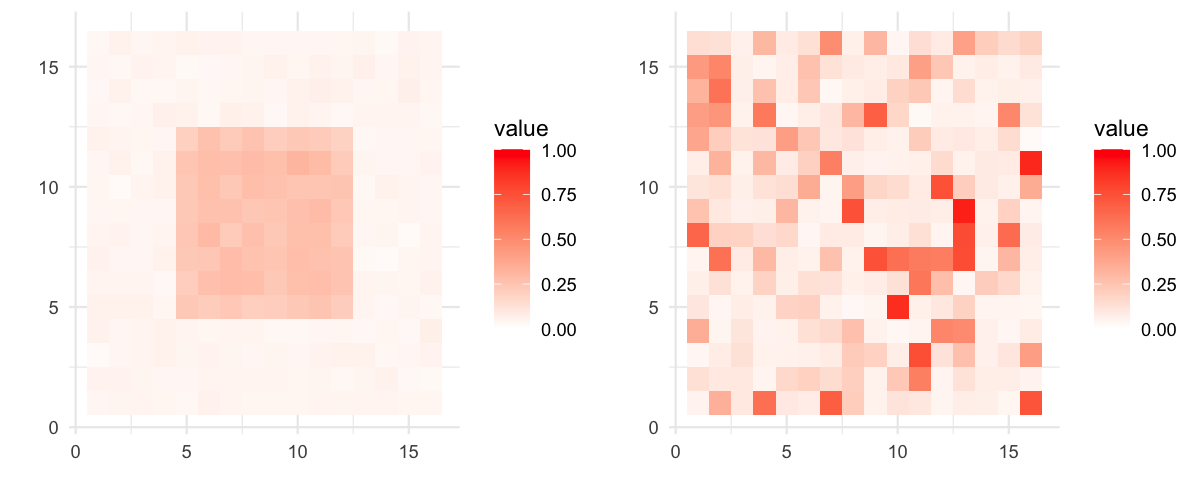
\includegraphics[width=0.9\textwidth]{perc_sign_pvals_hdi_beta.png}
	\caption{Percentage of significant p-values for elements of \( \beta \) when fitting models in the pixel space in
		Simulation 1 (left) and Simulation 2 (right).}
	\label{fig:perc_sign_beta}
\end{figure}

\begin{figure}[h!]
	\centering
	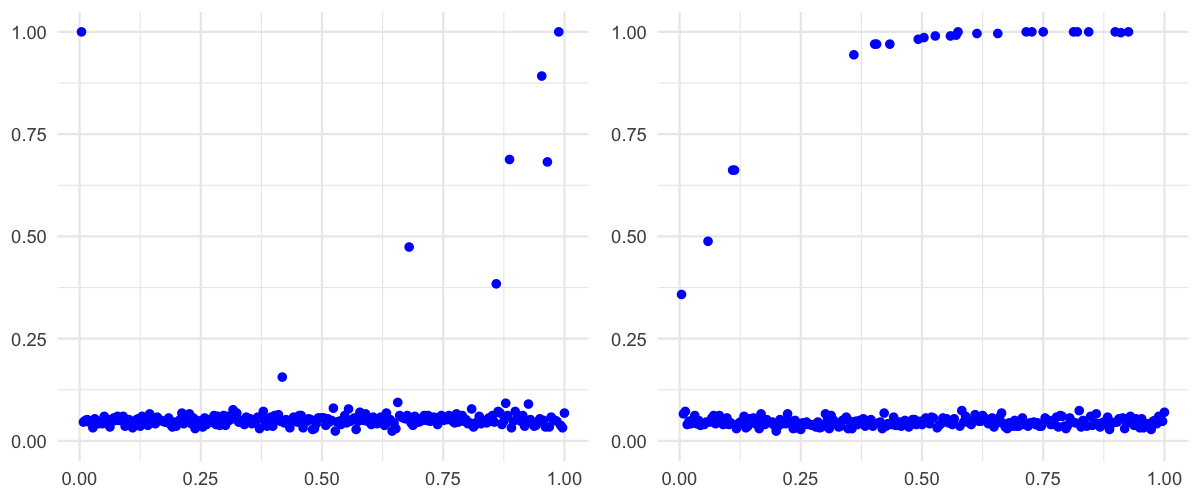
\includegraphics[width=0.9\textwidth]{perc_sign_pvals_hdi_b.png}
	\caption{Percentage of significant p-values for elements of \( b \) across ordered eigenvalues in both simulations.}
	\label{fig:perc_sign_b}
\end{figure}

\FloatBarrier

Figure~\ref*{fig:top_bottom_eigvecs} presents the frequencies associated with the top three eigenvalues, which represent the dominant patterns in the pixel space. The frequency associated with the smallest eigenvalue is also shown, highlighting the least significant variance.

\begin{figure}[h!]
	\centering
	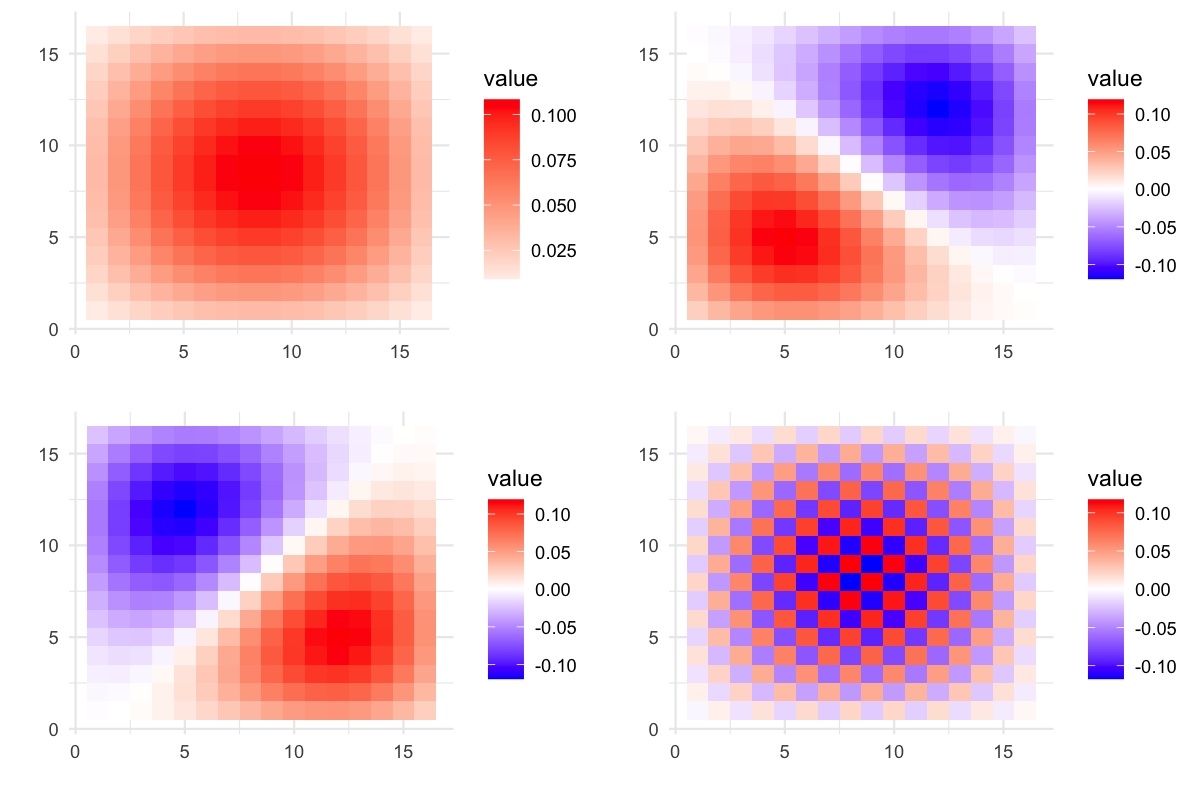
\includegraphics[width=0.8\textwidth]{top_bottom_eigvecs.png}
	\caption{Frequencies associated with the top three eigenvalues (top row and bottom left) and the frequency associated with the smallest eigenvalue (bottom right), highlighting the primary and least significant patterns in the pixel space.}
	\label{fig:top_bottom_eigvecs}
\end{figure}


\end{document}


Murakami and Griffith, “Eigenvector Spatial Filtering for Large Data Sets.”
